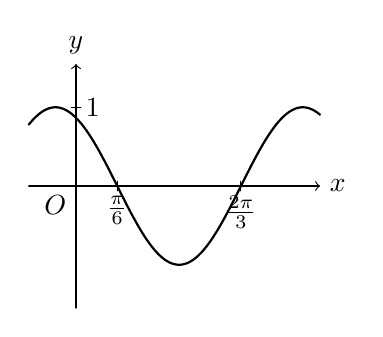
\begin{tikzpicture}[line cap=round,line join=round,scale=1]
\def\xmin{-0.6}
\def\xmax{3.1}
\def\ymin{-1.55}
\def\ymax{1.55}

\draw[->] (\xmin,0) -- (\xmax,0) node[right] {$x$};
\draw[->] (0,\ymin) -- (0,\ymax) node[above] {$y$};
\node[below left] at (0,0) {$O$};

\draw (-0.06,1) -- (0.06,1);
\node[right] at (0,1) {$1$};

\draw ({pi/6},-0.06) -- ({pi/6},0.06);
\node[below] at ({pi/6},0) {$\frac{\pi}{6}$};

\draw ({2*pi/3},-0.06) -- ({2*pi/3},0.06);
\node[below] at ({2*pi/3},0) {$\frac{2\pi}{3}$};

\draw[thick,domain=\xmin:\xmax,samples=200]
  plot (\x,{sin((pi/3-2*\x) r)});
\end{tikzpicture}